\documentclass[11pt, a4paper]{article}

% --- PACHETTI ESSENZIALI ---
\usepackage[utf8]{inputenc}    % Codifica input
\usepackage[T1]{fontenc}       % Codifica font output
\usepackage[italian]{babel}    % Lingua italiana
\usepackage{amsmath, amssymb}  % Simboli matematici
\usepackage{graphicx}          % Inclusione immagini
\usepackage{xcolor}            % Colori
\usepackage{hyperref}          % Link cliccabili (PDF)
\usepackage{geometry}          % Margini pagina
\usepackage{listings}          % Inclusione codice sorgente
\usepackage{fancyhdr}          % Intestazioni e piè di pagina personalizzati
\usepackage{enumitem}          % Personalizzazione elenchi
\usepackage{sectsty}           % Personalizzazione stile sezioni
\usepackage{tocloft}           % Personalizzazione Table of Contents
\usepackage{float}             % Migliore posizionamento float (figure, tabelle)
\usepackage{lmodern}           % Font Latin Modern (supporto per bold tt)
\usepackage{microtype}         % Miglioramenti tipografici
\usepackage{hypcap}            % Corregge i link hyperref alle figure

% --- IMPOSTAZIONI GEOMETRIA PAGINA ---
\geometry{
    a4paper,
    left=2.5cm,
    right=2.5cm,
    top=2.5cm,
    bottom=3cm,
    headheight=15pt
}

% --- IMPOSTAZIONI HYPERREF ---
\hypersetup{
    colorlinks=true,
    linkcolor=blue!70!black,
    citecolor=green!60!black,
    urlcolor=magenta!80!black,
    pdftitle={Report Progetto GCP: Chronicle-Sniffer},
    pdfauthor={Filippo Lucchesi},
    pdfsubject={Scalable and Reliable Services Project},
    pdfkeywords={GCP, Cloud Run, Pub/Sub, Terraform, Docker, TShark, UDM, Sniffer}
}

% --- STILE LISTINGS (CODICE) ---
\definecolor{codegreen}{rgb}{0,0.6,0}
\definecolor{codegray}{rgb}{0.5,0.5,0.5}
\definecolor{codepurple}{rgb}{0.58,0,0.82}
\definecolor{backcolour}{rgb}{0.98,0.98,0.98} % Sfondo leggermente grigio

% Definizione linguaggio HCL per Listings
\lstdefinelanguage{HCL}{
    morekeywords={resource,data,provider,variable,output,module,locals,terraform,source,project,name,location,template,service_account,image_uri,ports,env,resources,limits,cpu,memory,startup_probe,liveness_probe,http_get,path,dynamic,for_each,content,push_config,oidc_token,dead_letter_policy,depends_on,count,filter,metric_descriptor,labels,label_extractors,bucket_options,value_extractor,display_name,combiner,conditions,condition_threshold,duration,comparison,threshold_value,trigger,aggregations,alignment_period,per_series_aligner,cross_series_reducer,group_by_fields,notification_channels,documentation,mime_type,user_labels,machine_type,zone,boot_disk,initialize_params,image,network_interface,access_config,metadata,allow_stopping_for_update,network,allow,protocol,target_tags,source_ranges,uniform_bucket_level_access,versioning,encryption,lifecycle_rule,action,topic,ack_deadline_seconds,max_delivery_attempts},
    sensitive=false,
    morecomment=[l]{\#},
    morecomment=[s]{/*}{*/},
    morestring=[b]",
    morestring=[s]{<<EOT}{EOT},
    alsodigit={-}, % Permette '-' nei nomi delle keyword se necessario
}

\lstdefinestyle{mystyle}{
    backgroundcolor=\color{backcolour},
    commentstyle=\color{codegreen}\itshape,
    keywordstyle=\color{blue!80!black}\bfseries,
    numberstyle=\tiny\color{codegray},
    stringstyle=\color{codepurple},
    basicstyle=\ttfamily\footnotesize,
    breakatwhitespace=false,
    breaklines=true,
    captionpos=b,
    keepspaces=true,
    numbers=left,
    numbersep=5pt,
    showspaces=false,
    showstringspaces=false,
    showtabs=false,
    tabsize=2,
    frame=tb,
    framerule=0.4pt,
    rulecolor=\color{black!30},
    language=Python % Lingua di default
}
\lstset{style=mystyle}

% Stile specifico per HCL (Terraform)
\lstdefinestyle{hclstyle}{
    style=mystyle,
    language=HCL,
    keywordstyle=\color{orange!80!black}\bfseries
}

% Stile specifico per Bash
\lstdefinestyle{bashstyle}{
    style=mystyle,
    language=bash,
    keywordstyle=\color{red!80!black}\bfseries,
    morekeywords={echo,if,then,else,fi,for,do,done,while,case,esac,function,return,local,readonly,declare,export,unset,source,true,false,command,exit,trap,sleep,kill,wait,find,read,rm,gcloud,tshark,lsof,stat,basename,cut,grep,head,mv,sudo,cat,mkdir,chmod,systemctl,docker,apt-get,curl}
}

% Stile specifico per JSON
\lstdefinestyle{jsonstyle}{
    style=mystyle,
    language=JSON,
    stringstyle=\color{green!50!black},
    keywordstyle=\color{blue!70!black},
    basicstyle=\ttfamily\scriptsize,
    literate=
        *{0}{{{\color{blue!70!black}0}}}{1}
         {1}{{{\color{blue!70!black}1}}}{1}
         {2}{{{\color{blue!70!black}2}}}{1}
         {3}{{{\color{blue!70!black}3}}}{1}
         {4}{{{\color{blue!70!black}4}}}{1}
         {5}{{{\color{blue!70!black}5}}}{1}
         {6}{{{\color{blue!70!black}6}}}{1}
         {7}{{{\color{blue!70!black}7}}}{1}
         {8}{{{\color{blue!70!black}8}}}{1}
         {9}{{{\color{blue!70!black}9}}}{1}
}

% Stile sezioni (richiede \usepackage{sectsty})
\sectionfont{\Large\bfseries\color{blue!70!black}}
\subsectionfont{\large\bfseries\color{blue!60!black}}
\subsubsectionfont{\normalsize\bfseries\color{blue!50!black}}

% --- INTESTAZIONI E PIÈ DI PAGINA ---
\pagestyle{fancy}
\fancyhf{} % Pulisce header e footer
\fancyhead[L]{\small\textit{Chronicle-Sniffer Report}}
\fancyhead[R]{\small\textit{F. Lucchesi}}
\fancyfoot[C]{\thepage}
\renewcommand{\headrulewidth}{0.4pt}
\renewcommand{\footrulewidth}{0.4pt}

% --- SOMMARIO (con \usepackage{tocloft}) ---
\renewcommand{\cfttoctitlefont}{\hfill\Large\bfseries\hfill} % Titolo ToC
\renewcommand{\cftaftertoctitle}{\hfill}
\setcounter{tocdepth}{6} % Profondità del sommario (sezioni, sottosezioni, subsubsections)
\renewcommand{\cftbeforesecskip}{0.6ex} % Spazio prima delle sezioni nel ToC
\renewcommand{\cftbeforesubsecskip}{0.4ex}  % Spazio prima delle sottosezioni nel ToC
\renewcommand{\cftbeforesubsubsecskip}{0.3ex} % Spazio prima delle subsubsections nel ToC
\renewcommand{\cftsecfont}{\normalsize\bfseries} % Font sezioni nel ToC
\renewcommand{\cftsubsecfont}{\normalsize}      % Font sottosezioni nel ToC
\renewcommand{\cftsubsubsecfont}{\small}     % Font subsubsections nel ToC
\renewcommand{\cftsecpagefont}{\normalsize\bfseries} % Font numero pagina sezioni
\renewcommand{\cftsubsecpagefont}{\normalsize}      % Font numero pagina sottosezioni
\renewcommand{\cftsubsubsecpagefont}{\small}     % Font numero pagina subsubsections

\begin{document}

% --- PAGINA DEL TITOLO ---
\begin{titlepage}
    \centering
    \null\vfill
    {\Huge\bfseries Chronicle-Sniffer\par}
    \vspace{1em}
    {\LARGE A Scalable Wireshark-to-SecOps Pipeline on GCP\par}
    \vspace{3em}
    {\Large\bfseries Filippo Lucchesi\par}
    {\large \texttt{filippo.lucchesi@studio.unibo.it}\par}
    \vspace{2em} 
    {\large Scalable and Reliable Services M\par}
    {\large Università di Bologna\par}
    \vspace{1em}
    {\large 10 Giugno 2025\par} % Data di presentazione
    \vfill\null
\end{titlepage}

\thispagestyle{empty}
\clearpage
\tableofcontents
\clearpage
\pagestyle{fancy}


%----------------------------------------------------------------------------------------
%	SEZIONE 1: INTRODUZIONE
%----------------------------------------------------------------------------------------
\section{Introduzione}
\label{sec:introduzione}

Questo report descrive l'architettura, l'implementazione e le caratteristiche di un progetto sviluppato per il corso di "Scalable and Reliable Services M" presso l'Università di Bologna. 

Il sistema, denominato "Chronicle-Sniffer", realizza una pipeline di elaborazione dati di rete su Google Cloud Platform (GCP), con l'obiettivo primario di catturare pacchetti di rete (PCAP e PCAPNG), processarli in modo scalabile e affidabile, e trasformarli nel formato Unified Data Model (UDM) per successive analisi, tipicamente in contesti di sicurezza informatica, er esempio avvalendosi del Software Google SecOps.

Il progetto rappresenta una significativa evoluzione di un precedente lavoro concepito per il corso di Cybersecurity (Wireshark-to-Chronicle-Pipeline). Mentre la versione iniziale si concentrava sulla logica di conversione locale, questa iterazione si focalizza sulla creazione di un'infrastruttura cloud-nativa robusta, enfatizzando scalabilità, resilienza, gestibilità e osservabilità. Le tecnologie chiave impiegate includono servizi gestiti di GCP come Cloud Storage, Pub/Sub (con supporto per Dead-Letter Queue - DLQ), e Cloud Run per l'elaborazione serverless. L'intera infrastruttura è definita e gestita tramite Terraform, promuovendo l'approccio Infrastructure as Code (IaC), e include la definizione di una dashboard operativa personalizzata in Cloud Monitoring. I componenti software sono containerizzati con Docker. L'analisi del traffico di rete si avvale di TShark per la cattura e la conversione iniziale, mentre lo script Python \texttt{json2udm\_cloud.py} è stato reingegnerizzato per un parsing JSON efficiente in streaming e una mappatura UDM più dettagliata.

L'obiettivo è dimostrare la capacità di costruire un servizio distribuito che non solo risponda a requisiti funzionali specifici, ma che sia anche progettato per operare in maniera efficiente, robusta, sicura e altamente osservabile in un ambiente cloud.

%----------------------------------------------------------------------------------------
%	SEZIONE 2: ARCHITETTURA GENERALE
%----------------------------------------------------------------------------------------
\section{Architettura Generale}
\label{sec:architettura_generale}

Il sistema Chronicle-Sniffer è progettato come una pipeline \textit{event-driven}, che sfrutta diversi servizi GCP per orchestrare il flusso dei dati dalla cattura del traffico di rete fino alla sua trasformazione finale. L'architettura si articola attorno a componenti principali che interagiscono in modo asincrono, garantendo disaccoppiamento e resilienza.

\begin{figure}[!htbp]
    \centering
    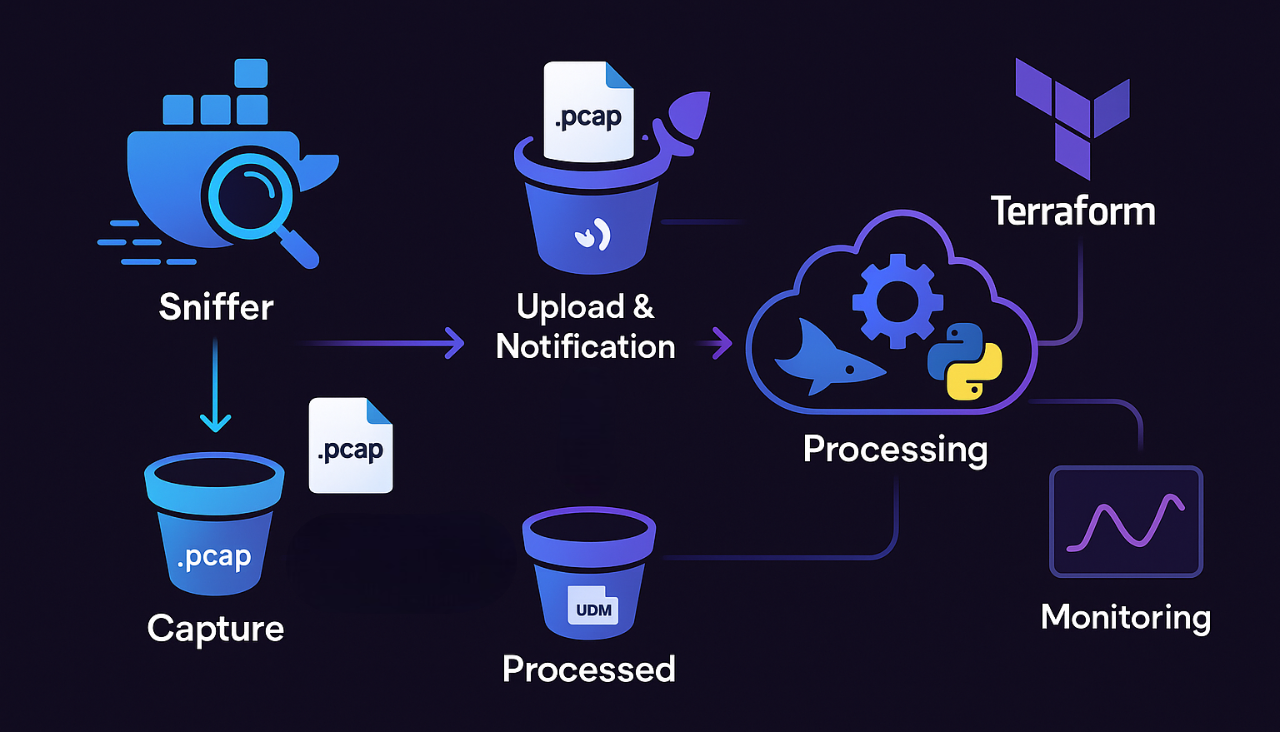
\includegraphics[width=0.9\textwidth]{pics/WORKFLOW.png}
    \caption{Diagramma dell'architettura generale del sistema Chronicle-Sniffer.}
    \label{fig:arch_diagram}
\end{figure}

\begin{itemize}[leftmargin=*, label=\textbullet]
    \item \textbf{Sniffer (On-Premises/Edge):} Un container Docker, eseguito su una macchina fisica o virtuale nell'ambiente da monitorare. Utilizza \texttt{tshark} per catturare il traffico di rete (supportando formati \texttt{.pcap} e \texttt{.pcapng}), gestisce la rotazione automatica dei file di cattura e, una volta completato un file, lo carica su un bucket Google Cloud Storage (GCS) (denominato \texttt{incoming-pcaps}). Immediatamente dopo, pubblica una notifica contenente il nome del file su un topic Google Cloud Pub/Sub. Lo sniffer include anche una funzionalità di \textit{heartbeat} per monitorarne lo stato.

    \item \textbf{Google Cloud Pub/Sub:} Agisce come \textit{message broker}. Un topic principale riceve le notifiche dallo sniffer. Una sottoscrizione \textit{push}, configurata con autenticazione OIDC sicura, inoltra i messaggi all'endpoint del servizio Cloud Run. È previsto un topic Dead-Letter Queue (DLQ) per gestire i messaggi che non possono essere processati correttamente dopo vari tentativi.

    \item \textbf{Google Cloud Storage (GCS):} Due bucket distinti sono utilizzati:
    \begin{itemize}
        \item \texttt{incoming-pcaps}: Funge da area di \textit{staging} per i file di cattura raw. Come visibile nello screenshot seguente (Figura~\ref{fig:gcs_incoming}), questo bucket riceve i file \texttt{.pcap} direttamente dallo sniffer.
        \begin{figure}[H]
            \centering
            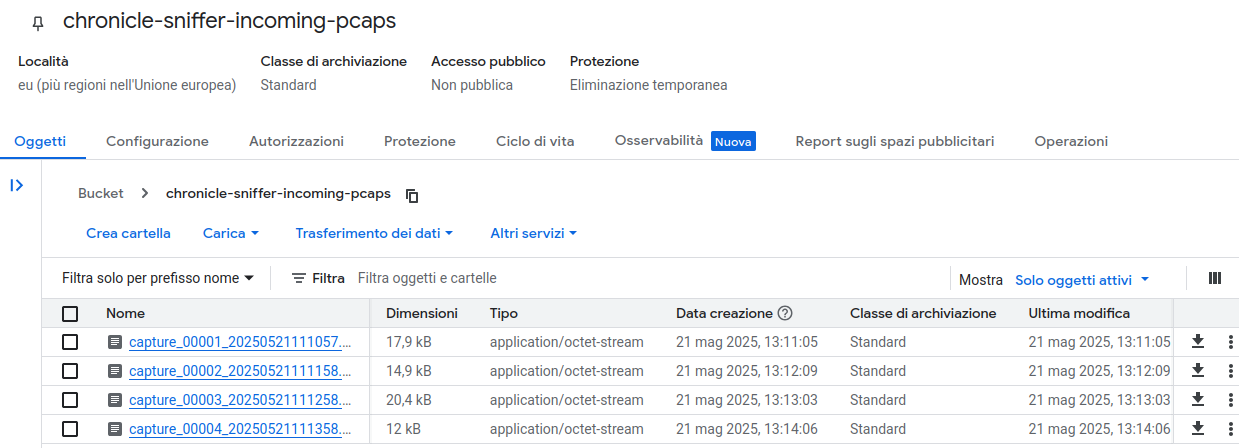
\includegraphics[width=0.9\textwidth]{pics/GCS_INCOMING_131510.png}
            \caption{Contenuto del bucket GCS \texttt{chronicle-sniffer-incoming-pcaps}.}
            \label{fig:gcs_incoming}
        \end{figure}
        \item \texttt{processed-udm}: Archivia i file JSON finali contenenti gli eventi di rete trasformati nel formato UDM. Lo screenshot successivo (Figura~\ref{fig:gcs_processed}) mostra un esempio dei file \texttt{.udm.json} prodotti dal Processor.
        \begin{figure}[H]
            \centering
            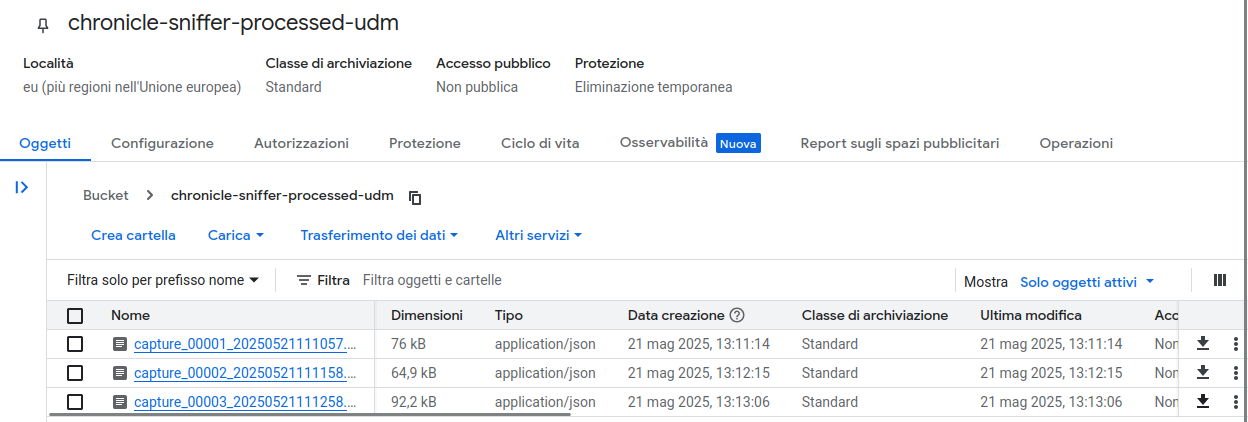
\includegraphics[width=0.9\textwidth]{pics/GCS_PROCESSED_131456.png}
            \caption{Contenuto del bucket GCS \texttt{chronicle-sniffer-processed-udm}.}
            \label{fig:gcs_processed}
        \end{figure}
    \end{itemize} 
    
    \item \textbf{Processore (Google Cloud Run):} Un servizio serverless che esegue un container Docker. Attivato dalle notifiche Pub/Sub, il servizio:
    \begin{enumerate}
        \item Scarica il file di cattura specificato da GCS.
        \item Utilizza \texttt{tshark} (installato nel container) per convertire il file di cattura in un formato JSON strutturato.
        \item Esegue lo script Python \texttt{json2udm\_cloud.py}, che ora utilizza la libreria \texttt{ijson} per il parsing in streaming del (potenzialmente grande) output JSON di \texttt{tshark}. Questo approccio è cruciale per l'efficienza della memoria in Cloud Run. Lo script mappa ogni pacchetto nel formato UDM.
        \item Carica il file UDM JSON risultante nel bucket GCS \texttt{processed-udm}.
    \end{enumerate}
    Il servizio è progettato per scalare automaticamente e include \textit{health probes} per il monitoraggio da parte di Cloud Run.
\end{itemize}

L'intera infrastruttura, inclusi i bucket, il topic Pub/Sub con DLQ, il servizio Cloud Run, i Service Account, i permessi IAM, le metriche basate su log e una dashboard operativa personalizzata, è definita e gestita tramite Terraform.

\subsection{Motivazioni delle Scelte Architetturali}
L'architettura è stata definita per massimizzare scalabilità, affidabilità, gestibilità, efficienza dei costi e sicurezza:
\begin{itemize}
    \item \textbf{Scalabilità:} Cloud Run e Pub/Sub scalano automaticamente per gestire carichi variabili. L'elaborazione in streaming nel Processor previene colli di bottiglia legati all'esaurimento della memoria.
    \item \textbf{Affidabilità e Resilienza:} Il disaccoppiamento tramite Pub/Sub, unito al supporto DLQ, garantisce che i messaggi non vengano persi e che i fallimenti siano gestiti in modo isolato. Cloud Run gestisce la disponibilità delle istanze del processor.
    \item \textbf{Gestibilità (IaC):} Terraform permette una gestione dichiarativa, versionabile e automatizzata dell'intera infrastruttura, inclusa la dashboard di monitoraggio.
    \item \textbf{Efficienza dei costi:} I servizi serverless e lo scaling a zero di Cloud Run ottimizzano i costi.
    \item \textbf{Sicurezza:} Adozione del principio del \textit{least privilege} per i Service Account, autenticazione OIDC tra Pub/Sub e Cloud Run, e gestione sicura delle chiavi per lo sniffer on-premises.
    \item \textbf{Osservabilità:} Integrazione profonda con Cloud Logging e Cloud Monitoring, con metriche personalizzate basate su log (LBM) e una dashboard operativa dedicata per una visione completa dello stato e delle prestazioni della pipeline.
\end{itemize}

%----------------------------------------------------------------------------------------
%	SEZIONE 3: LOGICA DI CONVERSIONE E ADATTAMENTO CLOUD
%----------------------------------------------------------------------------------------
\section{Logica di Conversione e Adattamenti per il Cloud}
\label{sec:logica_conversione}

Il cuore analitico del sistema è lo script Python \texttt{json2udm\_cloud.py}, eseguito dal componente Processor. Questo script è responsabile della trasformazione dei dati dei pacchetti, precedentemente convertiti in JSON da \texttt{tshark}, nel formato standardizzato Unified Data Model (UDM). È importante sottolineare che la logica dettagliata di parsing dei singoli campi PCAP e la loro mappatura iniziale ai concetti UDM sono state approfondite nel precedente progetto di Cybersecurity. Il focus di questo progetto è stato l'adattamento di tale logica per un ambiente cloud efficiente e la costruzione di un'infrastruttura scalabile e resiliente attorno ad essa.

\subsection{Evoluzione per l'Efficienza Cloud: da \texttt{json.loads} a \texttt{ijson}}
Nel progetto di Cybersecurity, la conversione JSON $\rightarrow$ UDM avveniva caricando l'intero output JSON di \texttt{tshark} in memoria tramite \texttt{json.loads()}. Sebbene funzionale per file di dimensioni moderate, questo approccio diventa proibitivo in un ambiente serverless come Cloud Run quando si trattano file PCAP di grandi dimensioni, che possono generare output JSON di svariati gigabyte, portando a errori di Out of Memory (OOM).

La modifica più significativa in \texttt{json2udm\_cloud.py} è l'adozione della libreria \texttt{ijson}. Questa libreria permette il parsing JSON in streaming: invece di caricare l'intero documento, \texttt{ijson} processa il file JSON in modo incrementale, leggendo e interpretando gli oggetti JSON (in questo caso, i singoli pacchetti) uno alla volta.

\begin{lstlisting}[language=Python, caption={Estratto da \texttt{json2udm\_cloud.py}: Utilizzo di \texttt{ijson} per lo streaming.}, label=lst:ijson_streaming, basicstyle=\ttfamily\scriptsize]
# Lo script apre il file JSON prodotto da tshark in modalita binaria ('rb').
# ijson.items(f_json, 'item') crea un iteratore che assume che il file JSON
# sia un array di oggetti alla radice. 'item' istruisce ijson a restituire
# (yield) ciascun elemento di questo array principale, uno alla volta.
# Questo permette di processare pacchetti individualmente senza caricare
# l'intero array di pacchetti (potenzialmente enorme) in memoria.
try:
    with open(json_file_path, 'rb') as f_json: # Modalita binaria per ijson
        json_packet_iterator = ijson.items(f_json, 'item') 
        for packet_data_dict in json_packet_iterator:
            # Ogni 'packet_data_dict' e' un dizionario Python
            # rappresentante un singolo pacchetto.
            udm_event = convert_single_packet_to_udm(packet_data_dict)
            udm_events_list.append(udm_event)
            processed_packet_count += 1
            # ... (logica per contare errori specifici per pacchetto)
except ijson.JSONError as e_ijson:
    # Gestisce errori se il file JSON non e' ben formato
    # o non e' un array alla radice.
    logging.error(f"ijson.JSONError while parsing streaming JSON from {json_file_path}: {e_ijson}...")
    return []
\end{lstlisting}
Questo approccio riduce drasticamente il picco di utilizzo della memoria, rendendo il processo di conversione adatto anche per istanze Cloud Run con risorse limitate e capace di gestire file di input molto grandi.

\subsection{Funzionamento Adattato dello script \texttt{json2udm\_cloud.py}}
Oltre al parsing in streaming, lo script \texttt{json2udm\_cloud.py} è stato migliorato per:
\begin{itemize}
    \item \textbf{Robustezza:} Ogni pacchetto in input produce un evento UDM, anche se si tratta di un evento minimo che segnala un errore di elaborazione per quel pacchetto. La conversione dei timestamp (\texttt{convert\_timestamp\_robust}) è più resiliente, con fallback all'ora corrente in caso di formati imprevisti, garantendo la conformità UDM.

    \begin{lstlisting}[language=Python, caption={Estratto da \texttt{json2udm\_cloud.py}: Funzione \texttt{convert\_timestamp\_robust}.}, label=lst:convert_timestamp, basicstyle=\ttfamily\scriptsize]
# Questa funzione tenta diverse strategie per parsare il timestamp fornito da tshark.
# Inizia con il formato piu comune (con microsecondi), poi tenta formati alternativi
# (es. senza microsecondi, pulendo stringhe di fuso orario comuni).
# Se tutte le conversioni falliscono, logga un warning e restituisce l'ora corrente
# in formato ISO 8601 UTC, assicurando che il campo 'event_timestamp' dell'UDM
# sia sempre presente e valido.
def convert_timestamp_robust(timestamp_str):
    if not timestamp_str:
        logging.warning(f"Timestamp string is missing or empty. Using current time as fallback.")
        return datetime.now(timezone.utc).isoformat(timespec='microseconds').replace('+00:00', 'Z')
    try:
        # Tentativo primario: formato standard di tshark con microsecondi
        dt_naive = datetime.strptime(timestamp_str[:26], "%b %d, %Y %H:%M:%S.%f")
    except ValueError:
        # Fallback: prova a pulire stringhe di fuso orario e a parsare senza microsecondi
        try:
            cleaned_ts = timestamp_str.split(" UTC")[0]
            # Altri tentativi di pulizia potrebbero essere aggiunti qui
            cleaned_ts = cleaned_ts.split(" Central European Summer Time")[0].strip()
            dt_naive = datetime.strptime(cleaned_ts, "%b %d, %Y %H:%M:%S")
        except ValueError as e_fallback: # e_fallback non usato, rimosso per pulizia warning
            logging.warning(f"Error converting timestamp '{timestamp_str}' ... Using current time.")
            return datetime.now(timezone.utc).isoformat(timespec='microseconds').replace('+00:00', 'Z')

    # Assicura che il datetime sia 'aware' (consapevole del fuso orario) e in UTC.
    dt_aware = dt_naive.replace(tzinfo=timezone.utc)
    # Formatta in ISO 8601, assicurando la 'Z' per Zulu time (UTC).
    iso_timestamp = dt_aware.isoformat(timespec='microseconds').replace('+00:00', 'Z')
    return iso_timestamp
    \end{lstlisting} 

    \item \textbf{Struttura UDM Allineata:} La struttura degli eventi UDM generati è stata raffinata per aderire più strettamente alle aspettative di sistemi come Chronicle, con sezioni \texttt{metadata}, \texttt{principal}, \texttt{target}, \texttt{network} (che può contenere \texttt{application\_protocol\_data} per HTTP, DNS, TLS, annidato sotto \texttt{network}) e \texttt{additional} ben definite.
    
    \begin{lstlisting}[language=Python, caption={Estratto da \texttt{json2udm\_cloud.py}: Struttura di un evento UDM.}, label=lst:udm_structure, basicstyle=\ttfamily\scriptsize]
# ... (all'interno di convert_single_packet_to_udm)
udm_payload = {
    "metadata": {
        "event_timestamp": event_timestamp,
        "product_name": "Wireshark TShark",
        "vendor_name": "Wireshark",
        "event_type": event_type, # Determinato dinamicamente
        "description": f"Packet capture. Protocols: {frame.get('frame.protocols', 'N/A')}..."
    }
}
# Le sezioni principal, target, network, about, application_protocol_data, additional
# vengono popolate e aggiunte a udm_payload solo se contengono dati effettivi.
# Esempio per la sezione 'principal':
cleaned_principal = clean_none_values(udm_principal) # clean_none_values rimuove chiavi con valore None
if cleaned_principal: udm_payload["principal"] = cleaned_principal
# ... logica simile per le altre sezioni ...
return {"event": udm_payload} # L'evento UDM finale e' incapsulato in un oggetto "event"
    \end{lstlisting} 

    \item \textbf{Estrazione Dati Migliorata:} Utilizzo di funzioni helper come \texttt{get\_nested\_value} per un'estrazione sicura dei valori da strutture JSON potenzialmente complesse (evitando \texttt{KeyError}) e \texttt{extract\_values\_from\_tshark\_section} per campi multi-valore (es. query DNS).
    \item \textbf{Logging Dettagliato:} Lo script produce log informativi, inclusi contatori di pacchetti processati ed errori (\texttt{UDM\_PACKETS\_PROCESSED}, \texttt{UDM\_PACKET\_ERRORS}), utili per il monitoraggio tramite le metriche basate su log (LBM).
\end{itemize}
Il processo di conversione per ogni pacchetto implica l'estrazione dei layer protocollari (frame, eth, ip, tcp, udp, dns, http, tls, etc.), la mappatura dei campi rilevanti nelle sezioni UDM appropriate, e la normalizzazione dei dati. La selezione dei campi mappati rimane focalizzata sulla rilevazione di minacce e anomalie di rete.

%----------------------------------------------------------------------------------------
%	SEZIONE 4: COMPONENTE SNIFFER
%----------------------------------------------------------------------------------------
\section{Componente Sniffer (Edge)}
\label{sec:sniffer}

Lo Sniffer è l'agente di cattura della pipeline, progettato per operare in ambienti on-premises o su dispositivi edge. È implementato come un container Docker leggero basato su Alpine Linux, contenente \texttt{tshark} e gli strumenti \texttt{gcloud}.

Il suo comportamento è orchestrato dallo script \texttt{sniffer\_entrypoint.sh}. All'avvio, lo script valida le variabili d'ambiente (ID progetto, bucket, topic, e un \texttt{SNIFFER\_ID} univoco), si autentica con GCP, e rileva automaticamente un'interfaccia di rete attiva (escludendo interfacce virtuali o di loopback). Avvia quindi \texttt{tshark} in background, configurato per la rotazione dei file di cattura (supportando estensioni \texttt{.pcap} e \texttt{.pcapng} tramite il pattern \texttt{*.pcap*}) in base a dimensione o tempo (configurabile tramite la variabile \texttt{ROTATE}).

\begin{lstlisting}[language=bash, style=bashstyle, caption={Estratto da \texttt{sniffer\_entrypoint.sh}: Avvio di \texttt{tshark}.}, label=lst:tshark_start, basicstyle=\ttfamily\scriptsize]
# La variabile $INTERFACE viene determinata automaticamente o presa dall'ambiente.
# $ROTATE definisce i criteri di rotazione (es., "-b filesize:10240 -b duration:60").
# $LIMITS puo' contenere filtri di cattura aggiuntivi.
# I file vengono scritti nella directory $CAPTURE_DIR con un nome base $FILENAME_BASE.
echo "(ID: $SNIFFER_ID) Starting tshark capture..."
tshark $INTERFACE $ROTATE $LIMITS -w "$CAPTURE_DIR/$FILENAME_BASE.pcap" &
TSHARK_PID=$! # Salva il PID di tshark per monitoraggio e shutdown.
echo "(ID: $SNIFFER_ID) tshark started with PID $TSHARK_PID"
\end{lstlisting} 
Un loop di monitoraggio verifica costantemente la presenza di file completati (non più attivamente scritti da \texttt{tshark}, identificati tramite \texttt{lsof}). Per ogni file completato, lo script ne logga la dimensione (\texttt{PCAP\_SIZE\_BYTES}), lo carica su GCS, pubblica una notifica con il nome del file su Pub/Sub, e infine rimuove il file locale. L'output dei log dello sniffer, come mostrato nello screenshot (Figura~\ref{fig:sniffer_logs}), evidenzia queste operazioni.

\begin{figure}[!htbp]
    \centering
    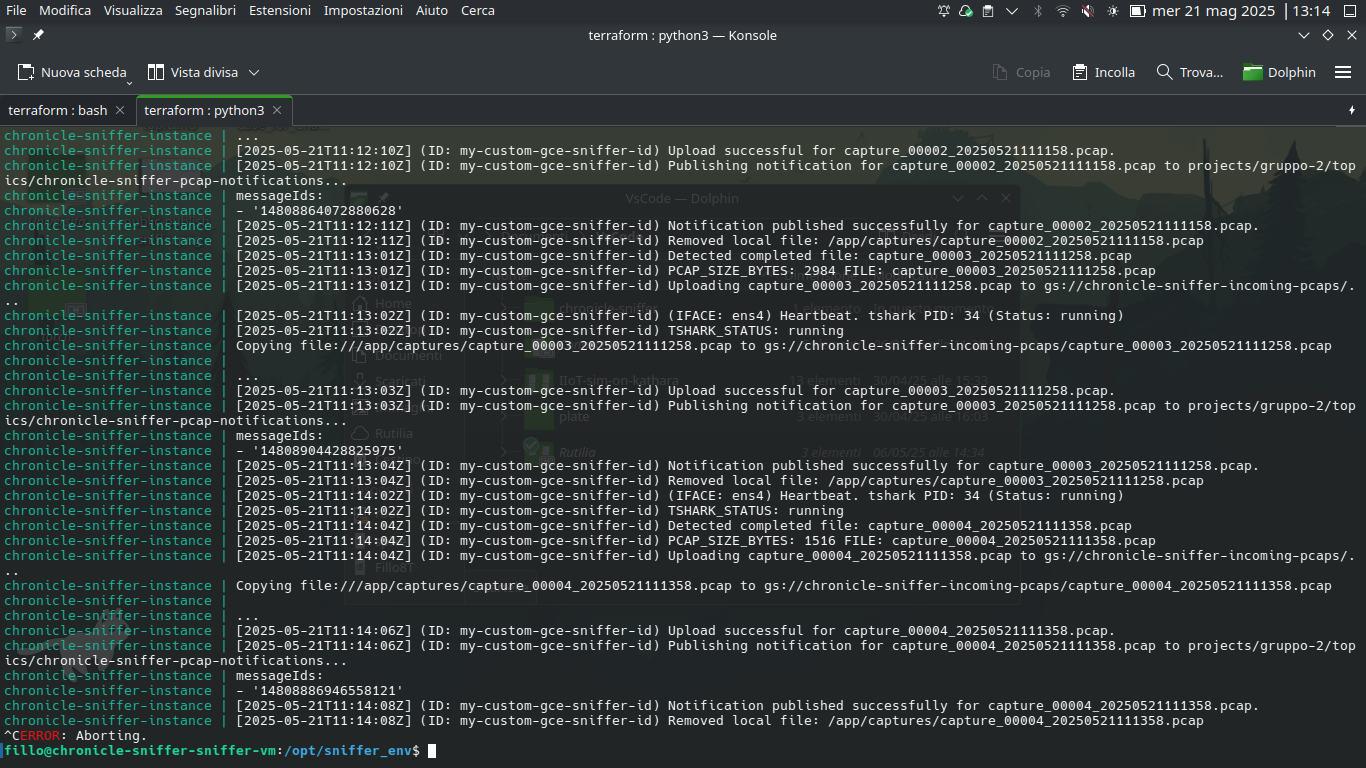
\includegraphics[width=0.8\textwidth]{pics/LOG_SNIFFER_131433.png}
    \caption{Log del container Sniffer durante l'upload e la notifica.}
    \label{fig:sniffer_logs}
\end{figure}

\begin{lstlisting}[language=bash, style=bashstyle, caption={Estratto da \texttt{sniffer\_entrypoint.sh}: Upload a GCS e notifica a Pub/Sub.}, label=lst:sniffer_upload_notify, basicstyle=\ttfamily\scriptsize]
# Questo blocco viene eseguito per ogni file PCAP completato.
# "$pcap_file_path" e' il percorso del file locale.
# "$current_pcap_file_basename" e' solo il nome del file.
echo "[$(date)] (ID: $SNIFFER_ID) Uploading $current_pcap_file_basename to gs://${INCOMING_BUCKET}/..."
if gcloud storage cp "$pcap_file_path" "gs://${INCOMING_BUCKET}/" --project "$GCP_PROJECT_ID"; then
    echo "[$(date)] (ID: $SNIFFER_ID) Upload successful for $current_pcap_file_basename."

    echo "[$(date)] (ID: $SNIFFER_ID) Publishing notification for $current_pcap_file_basename to ${PUBSUB_TOPIC_ID}..."
    if gcloud pubsub topics publish "$PUBSUB_TOPIC_ID" --message "$current_pcap_file_basename" --project "$GCP_PROJECT_ID"; then
        echo "[$(date)] (ID: $SNIFFER_ID) Notification published successfully for $current_pcap_file_basename."
        processed_files+=("$current_pcap_file_basename") # Aggiunge alla lista dei file processati.
        rm "$pcap_file_path" # Rimuove il file locale.
        echo "[$(date)] (ID: $SNIFFER_ID) Removed local file: $pcap_file_path"
    else
        # Errore nella pubblicazione Pub/Sub, il file non viene rimosso e verra' ritentato.
        echo "[$(date)] (ID: $SNIFFER_ID) Error: Failed to publish notification for $current_pcap_file_basename. Will retry."
    fi
else
    # Errore nell'upload GCS, il file non viene rimosso e verra' ritentato.
    echo "[$(date)] (ID: $SNIFFER_ID) Error: Failed to upload $current_pcap_file_basename to GCS. Will retry."
fi
\end{lstlisting} 
Lo script include una funzione di \textit{heartbeat} che logga periodicamente lo stato di \texttt{tshark} (\texttt{TSHARK\_STATUS: running/stopped}) e l'ID dello sniffer, facilitando il monitoraggio remoto della sua attività. Gestisce anche i segnali \textit{SIGTERM} e \textit{SIGINT} per un arresto pulito di \texttt{tshark}. La configurazione per l'avvio locale tramite \texttt{docker-compose} è fornita per facilitare test e sviluppo.

Un aspetto cruciale dello sniffer è il suo basso impatto sulle risorse del sistema edge. Come evidenziato dall'output del comando \texttt{docker stats} (vedi Figura~\ref{fig:docker_stats}), il container dello sniffer opera con un utilizzo minimo di CPU e memoria (nell'esempio, circa 0.05\% CPU e $\sim$100MB di RAM), rendendolo facilmente integrabile anche in ambienti con risorse limitate senza impattare significativamente le prestazioni di altri servizi. Questa efficienza è fondamentale per un'adozione su larga scala in contesti aziendali.

\begin{figure}[!htbp]
    \centering
    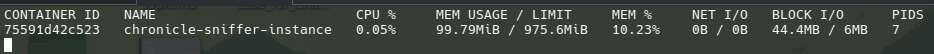
\includegraphics[width=0.8\textwidth]{pics/DOCKER_STATS_131634.png}
    \caption{Output di \texttt{docker stats} per il container Sniffer.}
    \label{fig:docker_stats}
\end{figure} 

%----------------------------------------------------------------------------------------
%	SEZIONE 5: COMPONENTE PROCESSOR
%----------------------------------------------------------------------------------------
\section{Componente Processor (Cloud Run)}
\label{sec:processor}

Il Processor, eseguito su Cloud Run, è il cuore dell'elaborazione. L'applicazione Flask \texttt{processor\_app.py} riceve le notifiche Pub/Sub. Una novità importante è la verifica "\textit{lazy}" dell'accessibilità ai bucket GCS all'avvio dell'istanza o alla prima richiesta, per gestire meglio eventuali ritardi nella propagazione dei permessi IAM post-deployment.

Per ogni notifica, l'applicazione scarica il file di cattura indicato, lo elabora in una directory temporanea, e orchestra le due fasi di conversione:
\begin{enumerate}
    \item PCAP $\rightarrow$ JSON: Esegue \texttt{tshark -T json} come subprocess.
    \item JSON $\rightarrow$ UDM: Esegue lo script \texttt{json2udm\_cloud.py} (anch'esso come subprocess) sull'output JSON di \texttt{tshark}.
\end{enumerate}
I log del servizio Cloud Run, visibili nello screenshot (Figura~\ref{fig:cloudrun_logs}), mostrano le fasi di conversione e l'eventuale upload del file UDM risultante.

\begin{figure}[!htbp]
    \centering
    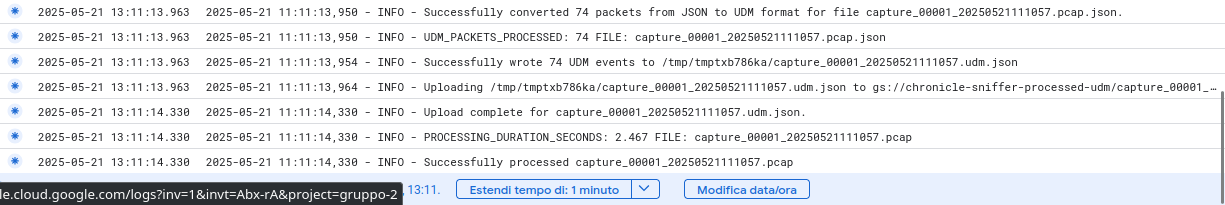
\includegraphics[width=\textwidth]{pics/LOG_PROCESSOR_131523.png}
    \caption{Log del servizio Cloud Run (Processor) durante l'elaborazione.}
    \label{fig:cloudrun_logs}
\end{figure}

\begin{lstlisting}[language=Python, caption={Estratto da \texttt{processor\_app.py}: Chiamata ai subprocess per \texttt{tshark} e \texttt{json2udm\_cloud.py}.}, label=lst:processor_subprocesses, basicstyle=\ttfamily\scriptsize]
# Questa logica viene eseguita all'interno di un blocco try...except per la gestione degli errori.
# local_pcap_path, local_json_path, local_udm_path sono percorsi in una directory temporanea.
try:
    # ... (download del file pcap da GCS) ...

    logging.info(f"Converting {local_pcap_path} to JSON...")
    tshark_command = ["tshark", "-r", local_pcap_path, "-T", "json"]
    # L'output JSON di tshark viene scritto direttamente su file.
    with open(local_json_path, "w") as json_file:
        # subprocess.run esegue il comando. check=True fa si che venga sollevata
        # un'eccezione CalledProcessError se tshark restituisce un exit code non zero.
        process = subprocess.run(tshark_command, stdout=json_file, stderr=subprocess.PIPE, text=True, check=True)
    logging.info(f"tshark conversion successful: {local_json_path}")
    if process.stderr: logging.warning(f"tshark stderr: {process.stderr.strip()}")

    logging.info(f"Converting {local_json_path} to UDM: {local_udm_path}")
    udm_script_command = ["python3", "/app/json2udm_cloud.py", local_json_path, local_udm_path]
    # Anche qui, check=True per catturare errori dallo script di conversione UDM.
    # capture_output=True per raccogliere stdout e stderr dello script.
    process = subprocess.run(udm_script_command, capture_output=True, text=True, check=True)
    logging.info(f"UDM conversion script done for {pcap_filename}.")
    if process.stdout: logging.info(f"json2udm_cloud.py stdout: {process.stdout.strip()}")
    if process.stderr: logging.warning(f"json2udm_cloud.py stderr: {process.stderr.strip()}")

    # ... (upload del file UDM a GCS) ...

except subprocess.CalledProcessError as e:
    # Gestisce errori specifici dei subprocess (tshark o json2udm_cloud.py).
    error_message = e.stderr.strip() if e.stderr else e.stdout.strip()
    logging.error(f"Subprocess error: CMD: {' '.join(e.cmd)} ERR: {error_message}", exc_info=False)
    return "Internal Server Error during processing step.", 500 # Segnala a Pub/Sub di ritentare.
# ... (altri blocchi except per errori GCS, etc.)
\end{lstlisting} 
L'applicazione logga la durata dell'elaborazione (\texttt{PROCESSING\_DURATION\_SECONDS}) per ogni file e gestisce gli errori restituendo codici HTTP appropriati a Pub/Sub per controllare i tentativi di acknowledgement (ack) o negative acknowledgement (nack).

%----------------------------------------------------------------------------------------
%	SEZIONE 6: INFRASTRUTTURA COME CODICE (TERRAFORM)
%----------------------------------------------------------------------------------------
\section{Infrastruttura come Codice (IaC) con Terraform}
\label{sec:iac_terraform}

L'intera infrastruttura GCP è gestita tramite Terraform. La configurazione è modulare e include:
\begin{itemize}
    \item Service Account dedicati con permessi minimi.
    \item Bucket GCS per i file di input e output.
    \item Topic Pub/Sub principale e un Dead-Letter Topic (DLQ), con una sottoscrizione \textit{push} verso Cloud Run configurata con autenticazione OIDC e una politica di \textit{dead-lettering}.
    \begin{lstlisting}[language=HCL, style=hclstyle, caption={Estratto da \texttt{terraform/main.tf}: Definizione della sottoscrizione Pub/Sub.}, label=lst:tf_pubsub_sub, basicstyle=\ttfamily\scriptsize]
resource "google_pubsub_subscription" "processor_subscription" {
  project              = var.gcp_project_id
  name                 = "${var.base_name}-processor-sub"
  topic                = module.pubsub_topic.topic_id # Topic principale
  ack_deadline_seconds = 600 # Tempo per Cloud Run per processare

  push_config {
    push_endpoint = module.cloudrun_processor.service_url # URL del servizio Cloud Run
    # Configurazione OIDC per l'autenticazione sicura
    dynamic "oidc_token" {
      for_each = !var.allow_unauthenticated_invocations ? [1] : []
      content {
        service_account_email = google_service_account.cloud_run_sa.email
        audience              = module.cloudrun_processor.service_url
      }
    }
  }

  # Politica per inviare messaggi non elaborabili al DLQ
  dead_letter_policy {
    dead_letter_topic     = module.pubsub_topic.dlq_topic_id # Topic DLQ
    max_delivery_attempts = 5 # Numero massimo di tentativi prima del DLQ
  }
  # ... (depends_on per gestione dipendenze)
}
    \end{lstlisting} 
    
    \item Servizio Cloud Run per il processor, con configurazione di immagine, variabili d'ambiente, risorse (CPU, memoria impostata a \texttt{2Gi} per gestire meglio \texttt{tshark}), concorrenza e \textit{health probes}.
    
    \begin{lstlisting}[language=HCL, style=hclstyle, caption={Estratto da \texttt{terraform/modules/cloudrun\_processor/main.tf}}, label=lst:tf_cloudrun_svc, basicstyle=\ttfamily\scriptsize]
resource "google_cloud_run_v2_service" "processor" {
  project  = var.project_id
  name     = var.service_name
  location = var.region

  template {
    service_account = var.service_account_email
    max_instance_request_concurrency = var.max_concurrency
    timeout                          = "600s" # Timeout per richiesta
    containers {
      image = var.image_uri
      ports { container_port = 8080 } # Porta interna del container
      dynamic "env" { # Passaggio dinamico delle variabili d'ambiente
        for_each = var.env_vars
        content {
          name  = env.key
          value = env.value
        }
      }
      resources { # Limiti di CPU e memoria per istanza
        limits = {
          cpu    = var.cpu_limit
          memory = var.memory_limit # Es. "2Gi"
        }
      }
      # Probe per monitorare la salute dell'applicazione
      startup_probe { http_get { path = "/" } # ... (configurazione dettagliata omessa per brevita) }
      liveness_probe { http_get { path = "/" } # ... (configurazione dettagliata omessa per brevita) }
    }
  }
  # ... (configurazione traffico omessa)
}
    \end{lstlisting}
    \item \textbf{Metriche Basate su Log (LBMs):} Definite in \texttt{terraform/main.tf} per tracciare eventi chiave come \textit{heartbeat} dello sniffer, upload di PCAP, errori di pubblicazione Pub/Sub, successo/fallimento delle conversioni \texttt{tshark}, pacchetti UDM processati/errori, e latenza di elaborazione. Queste metriche alimentano la dashboard operativa.
    \item \textbf{Dashboard Operativa:} Un file JSON (\texttt{terraform/dashboards/\allowbreak main\_operational\_dashboard.json}) definisce una dashboard completa in Cloud Monitoring utilizzando Monitoring Query Language (MQL). Questa dashboard visualizza le LBMs e le metriche standard dei servizi GCP, offrendo una visione centralizzata dello stato della pipeline. (Figure~\ref{fig:dashboard}).
    \begin{figure}[!htbp]
        \centering
        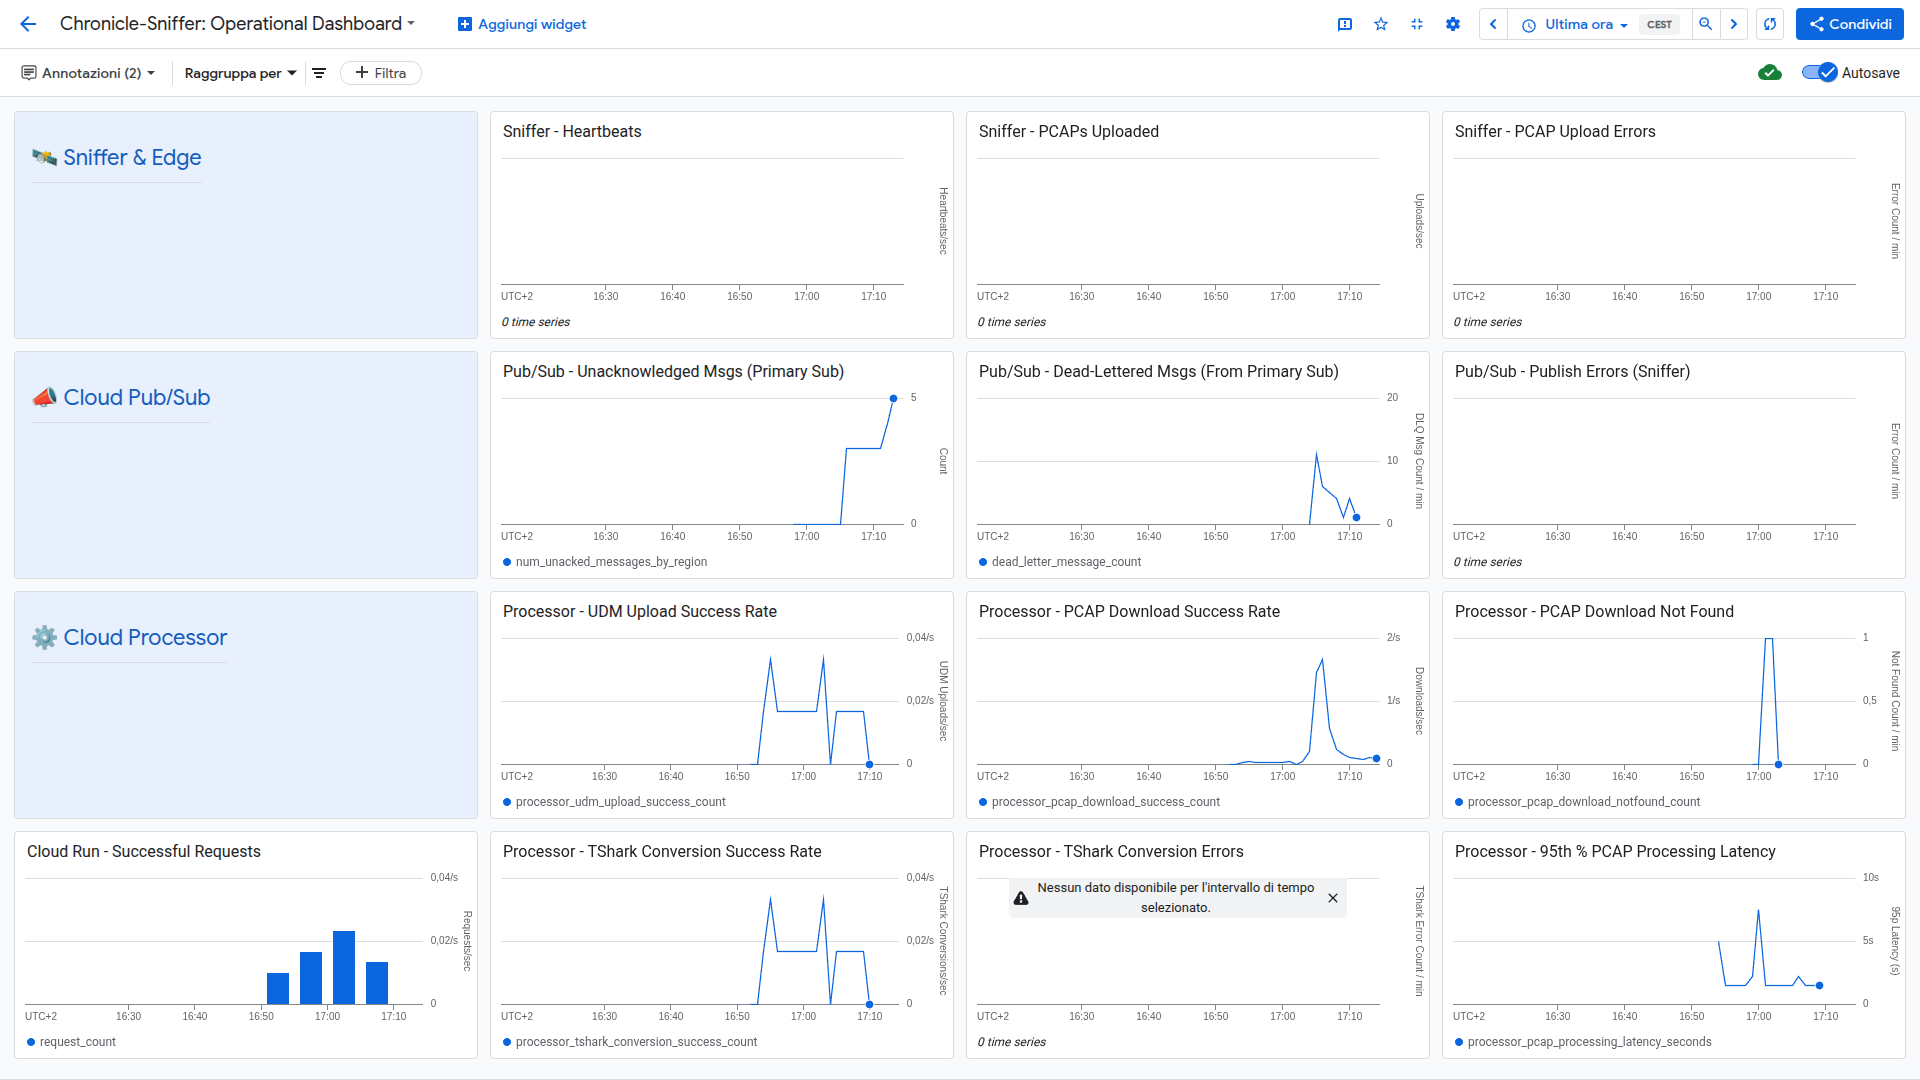
\includegraphics[width=0.9\textwidth]{pics/DASHBOARD.png}
        \caption{Dashboard Operativa in Cloud Monitoring.}
        \label{fig:dashboard}
    \end{figure} 
    
    \item \textbf{Politica di Alert (Esempio):} Una politica di alert di esempio per gli sniffer inattivi (basata sulla metrica di \textit{heartbeat}) dimostra come estendere l'osservabilità.
    \item \textbf{VM di Test (Opzionale):} Un modulo per creare una VM GCE che simula un ambiente on-prem, con uno script di avvio che prepara l'ambiente Docker Compose per lo sniffer.
\end{itemize}

%----------------------------------------------------------------------------------------
%	SEZIONE 7: VALORE DIDATTICO ED EVOLUZIONE
%----------------------------------------------------------------------------------------
\section{Valore Didattico ed Evoluzione del Progetto}
\label{sec:valore_didattico}

Questo progetto si distingue per la sua evoluzione da una soluzione locale a un'architettura cloud-nativa sofisticata. Il passaggio chiave è stato l'offloading dell'elaborazione intensiva al cloud e l'adozione di un design \textit{event-driven} e serverless. L'introduzione del parsing JSON in streaming (\texttt{ijson}) nello script \texttt{json2udm\_cloud.py} è un esempio di ottimizzazione per sfruttare a pieno l'ambiente cloud, dovuta ai limiti di memoria di Cloud Run. La definizione dell'intera infrastruttura e della dashboard di monitoraggio come codice (Terraform) sottolinea le moderne pratiche DevOps per la gestione di sistemi scalabili e affidabili. Il progetto dimostra l'applicazione pratica di concetti come disaccoppiamento, resilienza (DLQ), sicurezza IAM e osservabilità end-to-end. Le competenze acquisite includono la gestione di infrastrutture complesse con IaC, il design di sistemi serverless, il debugging in ambienti distribuiti e l'ottimizzazione delle risorse cloud.

%----------------------------------------------------------------------------------------
%	SEZIONE 8: ASPETTI OPERATIVI CHIAVE
%----------------------------------------------------------------------------------------
\section{Aspetti Operativi}
\label{sec:aspetti_operativi}
L'architettura progettata integra diversi meccanismi per garantire scalabilità, affidabilità, sicurezza e osservabilità, aspetti cruciali per un servizio operativo.

La \textbf{scalabilità} è gestita principalmente da Cloud Run, che adatta automaticamente il numero di istanze del Processor al carico di messaggi Pub/Sub, e dai servizi GCP sottostanti che scalano in modo trasparente.
L'\textbf{affidabilità} si basa sul disaccoppiamento fornito da Pub/Sub, che garantisce la persistenza dei messaggi e gestisce i tentativi di consegna in caso di fallimenti temporanei del Processor. Cloud Run contribuisce ulteriormente monitorando la salute delle istanze tramite \textit{health probes} e sostituendo quelle problematiche.
La \textbf{sicurezza} è implementata attraverso il principio del \textit{least privilege} per i Service Account, sull'autenticazione OIDC tra Pub/Sub e Cloud Run, la gestione delle chiavi SA on-premises e la configurazione sicura dei bucket GCS.
Infine, l'\textbf{osservabilità} è un punto di forza di questa versione evoluta. Oltre ai log centralizzati in Cloud Logging, il sistema si avvale di strumenti di monitoraggio avanzati:
\begin{itemize}
    \item \textbf{Metriche Basate su Log (LBMs):} Queste metriche, definite via Terraform, catturano eventi specifici dell'applicazione (es. \texttt{sniffer\_heartbeat\_count}, \texttt{pcap\_files\_uploaded\_count}, \texttt{processor\_pcap\_processing\_latency\_seconds}, \texttt{processor\_udm\_packets\_processed\_count}). Sono essenziali per comprendere il comportamento interno e le prestazioni della pipeline.
    \item \textbf{Dashboard Operativa Personalizzata:} Anch'essa gestita come codice (\texttt{json}) e deployata da Terraform, utilizza MQL per visualizzare sia le LBMs sia le metriche standard dei servizi GCP. Offre una visione d'insieme dello stato della pipeline, delle prestazioni dei singoli componenti (sniffer, Pub/Sub, processor) e dei tassi di errore, cruciale per la manutenzione proattiva e il troubleshooting.
\end{itemize}

%----------------------------------------------------------------------------------------
%	SEZIONE 9: TEST E VALIDAZIONE
%----------------------------------------------------------------------------------------
\section{Test e Validazione}
\label{sec:test_validazione}

La validazione della pipeline è facilitata dalla Test Generator VM, un componente cruciale dell'infrastruttura definita tramite Terraform. Questa VM non è semplicemente un ambiente di test generico, ma è concepita specificamente per simulare un ambiente on-premises o edge in cui lo sniffer opererebbe tipicamente. Questo ambiente simulato è fondamentale perché permette di replicare le condizioni operative reali del componente Sniffer, che è l'unico elemento della pipeline destinato a operare al di fuori dell'infrastruttura GCP gestita. Lo script di avvio della VM (\texttt{startup\_script\_vm.sh}) automatizza la configurazione di un ambiente Docker Compose completo, pronto per eseguire il container dello sniffer. In questo ambiente simulato, è possibile utilizzare strumenti come \texttt{tcpreplay} per "riprodurre" file PCAP preesistenti (ad esempio, un file illustrativo come \texttt{synflood\_capture.pcap} contenente traffico di un attacco simulato), immettendo traffico controllato nella rete della VM che verrà catturato dallo sniffer.

\begin{lstlisting}[language=bash, style=bashstyle, caption={Estratto da \texttt{terraform/modules/test\_generator\_vm/startup\_script\_vm.sh}.}, label=lst:tf_vm_startup, basicstyle=\ttfamily\scriptsize]
# Questo script, eseguito all'avvio della VM di test, automatizza la configurazione
# dell'ambiente per lo sniffer. Recupera i parametri necessari dai metadati dell'istanza
# (passati da Terraform) e crea i file di configurazione per Docker Compose.

# ... (installazione docker, pull immagine dello sniffer) ...

echo "Creating .env file for the sniffer in $SNIFFER_ENV_FILE"
# Il file .env conterra' le variabili d'ambiente specifiche per questa istanza
# dello sniffer sulla VM di test.
cat << EOF_ENV > "$SNIFFER_ENV_FILE"
GCP_PROJECT_ID=$VM_GCP_PROJECT_ID_FROM_METADATA
INCOMING_BUCKET=$VM_INCOMING_BUCKET_FROM_METADATA
PUBSUB_TOPIC_ID=$VM_PUBSUB_TOPIC_ID_FROM_METADATA
SNIFFER_ID=\${VM_SNIFFER_ID_FROM_METADATA}
# GCP_KEY_FILE e' ${SNIFFER_GCP_KEY_CONTAINER_PATH}/key.json
GCP_KEY_FILE=\${SNIFFER_GCP_KEY_CONTAINER_PATH}/key.json # Path interno al container
EOF_ENV

# ... (creazione di docker-compose.yml e docker-compose.override.yml specifici per la VM) ...
# L'override.yml gestisce il montaggio della chiave SA e della directory delle catture.
\end{lstlisting}
In aggiunta, per testare la reazione del sistema a scenari di traffico specifici o attacchi simulati, è possibile installare e utilizzare sulla VM strumenti come \texttt{hping3}. Ad esempio, un attacco SYN flood può essere simulato per osservare come i pacchetti anomali vengono catturati, processati e rappresentati nel formato UDM.
\begin{lstlisting}[language=bash, style=bashstyle, caption={Esempio di comando \texttt{hping3} per simulare un SYN flood (da eseguire sulla VM di test)}, label=lst:hping3_example, basicstyle=\ttfamily\scriptsize]
# Questo comando invia un gran numero di pacchetti TCP SYN alla porta 80
# dell'IP target, simulando l'inizio di molte connessioni senza completarle.
sudo hping3 -S --flood -p 80 <IP_TARGET_NELLA_RETE_DELLA_VM>
\end{lstlisting} 

Questa capacità di simulare un ambiente on-premises realistico, completo di strumenti per la generazione e la riproduzione di traffico, è fondamentale per validare end-to-end il funzionamento della pipeline e per osservarne il comportamento in condizioni controllate, inclusa la risposta a potenziali minacce di rete. File di esempio come un ipotetico \texttt{synflood\_capture.pcap} e il corrispondente \texttt{synflood\_capture.udm.json} servirebbero come riferimento per questa validazione.

%----------------------------------------------------------------------------------------
%	SEZIONE 10: CONCLUSIONI E SVILUPPI FUTURI
%----------------------------------------------------------------------------------------
\section{Conclusioni e Sviluppi Futuri}
\label{sec:conclusioni}

Questo progetto ha raggiunto l'obiettivo di evolvere una semplice utility di conversione in una pipeline di analisi del traffico di rete robusta, scalabile, osservabile e gestita come codice su GCP. L'adozione di tecniche come il parsing in streaming, l'architettura \textit{event-driven} con DLQ, e l'osservabilità tramite dashboard IaC dimostrano una comprensione matura dei principi per la creazione di servizi cloud affidabili.\\

Possibili sviluppi futuri includono:
\begin{itemize}
    \item Implementazione di test automatici di integrazione e unitari.
    \item Integrazione diretta con l'API di ingestion di \textit{Chronicle Security Operations} (\textit{Google SecOps}).
\end{itemize} 

Il sistema attuale, tuttavia, costituisce una solida piattaforma per l'analisi del traffico di rete su scala.
\newpage

%----------------------------------------------------------------------------------------
%	SEZIONE 11: BIBLIOGRAFIA E SITOGRAFIA ESSENZIALE
%----------------------------------------------------------------------------------------
\section{Bibliografia e Sitografia}
\label{sec:bibliografia}

\begin{thebibliography}{99}
    \bibitem{lucchesi2025} Lucchesi, Filippo (2025). \textit{chronicle-Sniffer}. GitHub Repository. \url{https://github.com/fillol/chronicle-sniffer} (Codice Sorgente)
    \bibitem{lucchesi2024} Lucchesi, Filippo (2024). \textit{Wireshark-to-Chronicle-Pipeline}. GitHub Repository. \url{https://github.com/fillol/Wireshark-to-Chronicle-Pipeline} (Progetto originario di Cybersecurity)
    \bibitem{dockerhub} Immagine Sniffer su Dockerhub. \url{https://hub.docker.com/r/fillol/chronicle-sniffer}
    \bibitem{gcp_run} Google Cloud. Cloud Run. \url{https://cloud.google.com/run/docs}
    \bibitem{gcp_pubsub} Google Cloud. Pub/Sub. \url{https://cloud.google.com/pubsub/docs}
    \bibitem{gcp_storage} Google Cloud. Cloud Storage. \url{https://cloud.google.com/storage/docs}
    \bibitem{gcp_udm} Google Cloud. Unified Data Model (UDM). \url{https://cloud.google.com/chronicle/docs/unified-data-model/udm-overview}
    \bibitem{gcp_monitoring} Google Cloud. Cloud Monitoring. \url{https://cloud.google.com/monitoring/docs}
    \bibitem{gcp_iam} Google Cloud. Identity and Access Management (IAM). \url{https://cloud.google.com/iam/docs}
    \bibitem{secops} Google SecOps. Chronicle \url{https://cloud.google.com/security/products/security-operations}
    \bibitem{terraform_docs} Terraform by HashiCorp. \url{https://developer.hashicorp.com/terraform/docs}
    \bibitem{docker_docs} Docker. \url{https://docs.docker.com/}
    \bibitem{tshark_man} TShark Manual Page. \url{https://www.wireshark.org/docs/man-pages/tshark.html}
    \bibitem{ijson_pypi} Python Software Foundation. ijson \url{https://pypi.org/project/ijson/}
    \bibitem{hping3_ref} Hping3. \url{https://www.kali.org/tools/hping3/}
    \bibitem{tcpreplay_man} Tcpreplay Manual Page. \url{https://tcpreplay.appneta.com/wiki/tcpreplay-man.html}
\end{thebibliography}

\end{document}